\chapter{Implémentation}
\label{ch:impl}

\section{Choix d'implémentations}
\subsection{Langage}
Au départ le choix du langage s'est porté sur sagemath (framework python) afin de mieux comprendre les différents calculs et faire un premier POC du chiffrement.
Cependant l'implémentation du POC était lente et le changement d'algorithme pour les pairings était difficile.
Je me suis donc orienté sur le C pour avoir de meilleures performances et pouvoir mieux gérer ma mémoire car c'est un point important dans des logiciels implémentant de la cryptographie. Pour pouvoir faire facilement des calculs sur les courbes elliptiques et les pairings en C il me fallait une librairie.
\subsection{Librairie}
La librairie utilisée est RELIC Toolkit~\cite{relic-toolkit}, c'est une librairie en cours de développement qui se veut efficiente. Sa concurrence avec MIRACL m'a fait hésiter dans mon choix, mais MIRACL est plus codée en C++ avec des équivalences en C j'ai donc choisi RELIC.
\subsection{Courbe utilisée}
La courbe utilisée pour le POC est la BLS12-P381, en effet cette courbe est assez efficiente et compatible avec les pairings. De plus RELIC l'a dans ses options et fonctionne bien, elle a un niveau de sécurité de 128bits. Je voulais prendre une courbe avec une plus grande sécurité cependant RELIC ne l'a pas encore totalement implémenté (certains tests ne passes pas), mais la librairie étant toujours en cours de développement il faudrait suivre ça de près, le code ne changerait en effet pas.
\subsection{Dérivation de la clé AES}
Le but de mon schéma certificateless est de chiffrer et signer une clé AES qui permettra à mon message d'avoir un chiffrement authentifié. Pour cela il me faut dériver un élément de Gt en clé AES.\\
Pour cela j'ai utilisé une fonction permettant d'écrire sous forme compressée mon élément en bytes. Puis j'ai effectué un hachage avec SHA256 dessus, ainsi le résultat du hachage est une clé AES-256. La fonction de hachage doit être par conséquent cryptographiquement sûre.
\subsection{Fonctions de hachage - signature}
Pour le schéma de signature il nous faut plusieurs fonctions de hachage différentes (3 en fait). Pour appliquer cela j'ai utilisé la même méthode de mapping disponible ans RELIC pour mapper une char array (tableau de byte) à un point sur G2 à savoir g2\_map.
Pour H1, la première fonction de hachage j'ai simplement utilisé cette fonction directement, mais pour H2 et H3 j'ai ajouté un byte devant les données à mapper respectivement les bytes '01' et '02'. Ceci afin de différencier les hash générés. Ceci s'appelles du 'Domain Hash Separation'.
\subsection{Sérialisation des données}
Pour la sérialisation des données, typiquement les clés publiques et les clés privées partielles envoyées en réseau ou les clés publiques enregistrées dans les fichiers par exemple, j'ai utilisé la librairie binn\footnote{\url{https://github.com/liteserver/binn}}. Cela permet de packer facilement des données binaires, pour cela RELIC met à disposition des méthodes g1\_write\_bin g1\_read\_bin qui a permis de faire ces enregistrements binaires. Ainsi les transferts de données sont simplifiés.
\subsection{Enregistrement des clés publiques}
Pour les enregistrements et récupération des clés publiques pour le KGC j'ai simplement mis en place une structure de fichiers simples : un dossier signature et un encryption. De là je crée un fichier par utilisateur avec leur ID comme nom de fichier, et met la clé publique dedans, ainsi lorsque l'on doit récupérer des clés publiques c'est assez simple à retorouver les clés. 
\section{Implémentation clés  de chiffrement}
Pour pouvoir implémenter ce schéma de chiffrement et signature certificateless dans un système hybride il a fallu penser à une manière d'encapsuler la clé et les données envoyées. Pour cela j'ai essayé de faire un système comparable à la figure \ref{fig:encapsulate}. L'on voit les données qui seront envoyées au destinataire et en fonction de quoi elles sont crées.
\begin{figure}[h!]
	\centering
	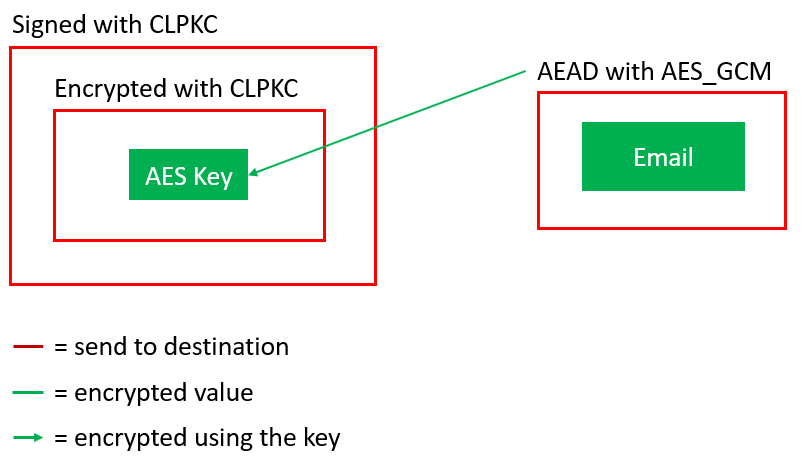
\includegraphics[width=12cm]{images/schemaEncapsulation.png}
	\caption{Schéma encapsulation des données}
	\label{fig:encapsulate}
\end{figure}

\subsection{Déroulement POC}
Je mets ici temporairement le code du main afin de voir le déroulement global d'un é change et voir ce qui a été implémenté jusque là.
\inputminted[linenos, numbersep=4pt,fontsize=\footnotesize, breaklines=true]{C}{source_code/main.c}